% Point out that for the first time in the literature Cartan's moving frame method is used to assess damage in infarcted hearts by looking at the degree to which fiber orientations in a local neighborhood of a voxel are consistent with its 1-form characterization. Point out that this parametric approach also leads to a geometric model for fibers in healthy regions. Point out that regions of high error explain more than 80\% of those regions with high ADC. However, they also include regions near the heart wall (endothilial and epithilial) linings. Talk about the promise of Cartan frame fitting error in the early stages post infart, not just after 4-6 week period which has been our current focus.

\chapter{Experimental Setup}

The data on which our results are based are all porcine hearts that were gratefully provided to us by Mihaela Pop from the Sunnybrooke University.

\section{Data acquisition of pig infarcted and healthy hearts}

Each porcine heart studied in this thesis were freshly excised, suspended in a plexiglass phantom filled with fluorinert (to eliminate artifacts) and placed in an MR head coil for ex-vivo imaging. All DW-MR studies were performed on a dedicated 1.5T GE Signa Excite scanner using a custom FSE pulse sequence. They used the following MR parameters: 
\begin{itemize}
    \item $TE = 35$ ms
    \item $TR = 700$ ms
    \item echo train length $=2$
    \item $b = 0$ for the unweighted MR images. As a reminder, the b factor is explained in \ref{dw_imaging}
    \item $b = 500 $ s/$\text{mm}^2$ for the images where the 7 diffusion gradients were applied
    \item $256 \times 256$ k-space
    \item Field of View $FOV = 10-16$ cm
    \item Slice Thickness $ = 1.2$ mm, yielding a sub-millimetric voxel size
\end{itemize}
From each heart, select samples containing an infarct were cut to align with the short-axis view of the MR images and prepared for histopathology to confirm the collagen deposition in the infarct area. One of the difficulties that remains is to try and find a good correspondence between the slices from the histology and the ones that were obtained from the imaging that occured before the histopathology was performed.  \ref{fig:histology_pig_4} shows a histology image of a slide from an infarcted heart, with intact myocytes in the normal tissue and altered tissue microstructure in the infarcted zone. As depicted by the Masson Trichrome stain, the ischemic border zone (BZ) had collagen fibrils interdigitated between viable myocytes. In the dense scar area, necrotic myocytes were completely replaced by mature fibrosis (the final product of collagen degradation), resulting in the loss of myocardial anisotropy.\\\\\\

\begin{figure}[h!]
    \centering
    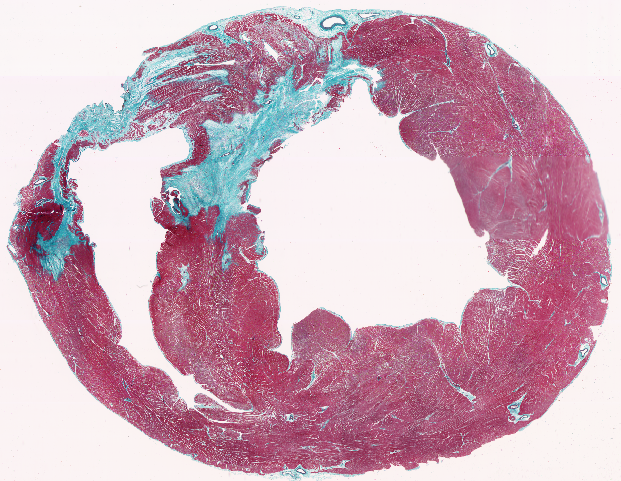
\includegraphics[width=\textwidth]{figures/Gip4_histology}
    \caption{Histology of a slice of infarcted heart nb 4}
    \label{fig:histology_pig_4}
\end{figure}

\section{Source of input data}

The data we have been using are DT-MRI of porcine hearts, both healthy for comparison and infarcted. We have had access to 10 hearts including 2 healthy. For every infarcted heart, the imaging process took place 6 weeks after infarct and histology was done after that for some of the cases - as it is an expensive process - which allows us to compare our observations to the ground truth. Here is an overview of the data we had access to and its usability:

\begin{center}
    \begin{tabular}{|c | c | c | c|} 
         \hline
         Heart (Acquisition Date) & Infarcted or Healthy & Region of infarct \\
         \hline
         2 & Infarcted & Left Circumflex artery (LCX) \\ 
         \hline
         4 & Infarcted & Left Anterior Descending (LAD) \\
         \hline
         5 & Infarcted & LCX \\
         \hline
         6 & Infarcted & LCX \\
         \hline
         7 & Infarcted & Rigth Coronary Artery (RCA) \\ 
         \hline
         17 & Infarcted & Bad quality \\
         \hline
         18 & Infarcted & Bad quality \\
         \hline
         23 & Infarcted & Unreadable \\
         \hline
         25 & Healthy & - \\
         \hline
         28 & Healthy & Too Noisy \\
         \hline
    \end{tabular}
\end{center}

\section{Quality of our data}

For a better and more accurate analysis of our results, we will focus mostly on the best quality data (least noisy) we had access to and fortunately those include one control heart (\#5: \ref{fig:pig25}) and 5 infarcted hearts (\#2: \ref{fig:pig2}, \#4: \ref{fig:pig4}, \#5: \ref{fig:pig5}, \#6: \ref{fig:pig6}, \#7: \ref{fig:pig7}). \\
Due to the imaging technology used, and to the fact that a fairly low Tesla intensity was used to acquire this data (1.5T), a good amount of noise is present in the raw data. We have taken advantage of the knowledge on the type of noise (Rician noise) that is present in MRI-acquired data to apply non-local denoising strategies which are a bit expensive in time but can smooth rather efficiently and not by too much the data to be able to have a better readability of the fiber orientation without oversmoothing. This prevents this strategy from smoothing even regions where the data is chaotic due to the infarct or proximity to the boundary and not only because of noise issues from acquisition. A fine tuning of the smoothing strategy allowed us to get good quality datasets without removing relevant information in the regions of interest around the infarcts.

\section{Usage of MedInria software to read the DICOMs}

We took the advantage of the MedInria tool to load the DICOM images, process the data through the Rician denoising method and finally use their Diffusion Tensor Imaging tool to compute the value of the tensor matrix at each voxel location in the heart. \\
From the tensor matrices at every location, we were easily able to compute the fiber orientation at every location with a potential flip in the sense of the vector. Cylindrical consistency was used to enforce a consistent sense throughout the heart. \\
Once we have the fiber orientation at every voxel, we can use our previous work to compute the connection forms and get an approximative appreciation of the quality of the fitting, depending on hyper parameters that have to be fine tuned by mostly on the coherence of the underlying data.